\documentclass[my_thesis.tex]{subfiles}

\begin{document}
\cleardoublepage
\chapter{Introduction}
\markboth{Introduction}{Introduction}
\addcontentsline{toc}{chapter}{Introduction}
 

Our civilization needs a new source of energy, and it needs to be nuclear fusion energy. In this introduction, we motivate this statement by looking at why energy is a crucial ingredient of human development. We discuss the available energy sources today, their advantages and disadvantages, and introduce the nuclear fusion reaction. We then focus on the stellarator, which is a nuclear fusion power plant concept which uses 3-dimensional magnetic fields to confine a plasma.

\section{Energy consumption and quality of life}

The Human Development Index (HDI)  \citep{undpunitednationsdevelopmentprogrammeHumanDevelopmentReport1990} is a composite statistic used to rank countries by their level of human development. It was developed by the United Nations Development Programme (UNDP) as an alternative to traditional measures of development, such as gross domestic product (GDP), which do not take into account other important dimensions of well-being such as health, education, and living standards. The HDI is a measure of the average achievements of a country in these three dimensions, calculated using life expectancy at birth, mean years of schooling, and gross national income per capita.

On Figure \ref{fig.hdi}, we show the HDI as a function of the average energy consumption per inhabitant, for a wide range of different countries. The HDI data were obtained from the UNDP website\footnote{\url{hdr.undp.org}, consulted the 26.12.2022}, while the energy consumption in each country and its number of inhabitant were obtained from the World Bank website\footnote{\url{data.worldbank.org}, consulted the 26.12.2022}. The data dates from 2014; at the time of writing this thesis, there were no extensive dataset that postdates 2014. One striking observation is that the HDI grows with the energy consumption per inhabitant --- in other words, the more energy is available, the higher the quality of life is.

\begin{figure}
    \centering
    \subfloat{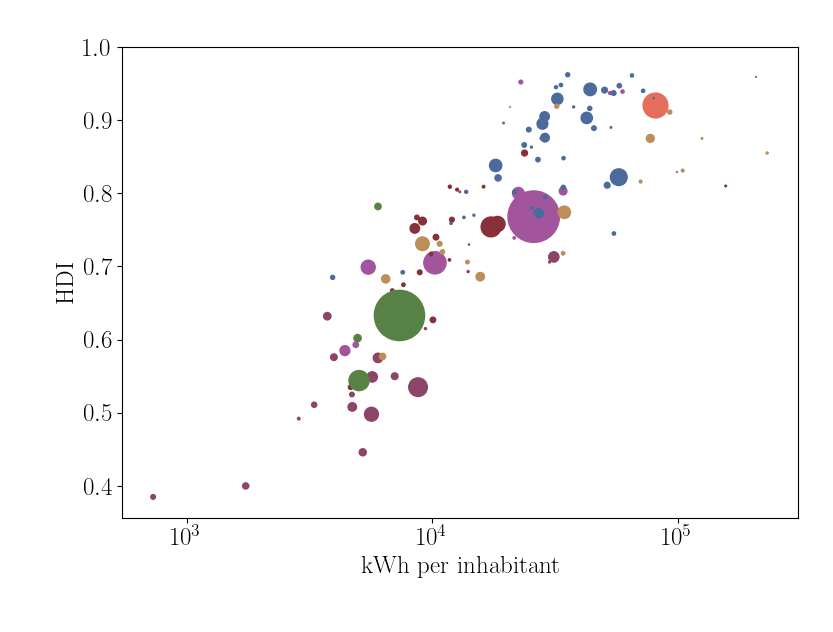
\includegraphics[width=\linewidth]{images/HDI_fct_kWh.png}}\\
    \centering
    \subfloat{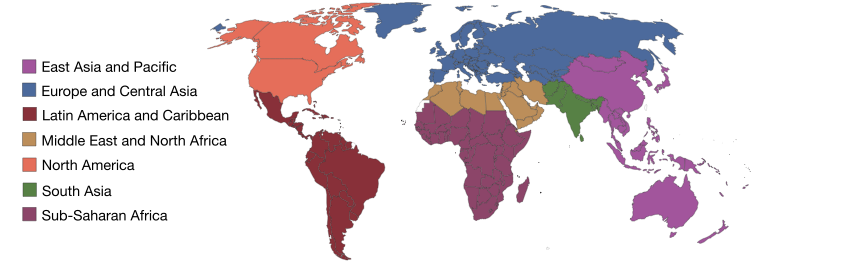
\includegraphics[width=\linewidth]{images/WorldMap.png}}
    \caption{Top: HDI as a function of the average energy consumption per country's inhabitant. Size of dots are proportionals to the total population of the country. Colors indicate the region the country belongs to, according to the World Bank classification. Bottom: regions defined by the World Bank classification.}
    \label{fig.hdi}
\end{figure}

Indeed, countries with the higher HDI are often the most developed. Energy is a critical factor in human development because it plays a vital role in supporting economic growth and improving people's quality of life. Access to energy allows people to participate in economic activities, access education and healthcare, and improve their living standards. For example, access to electricity can enable people to use appliances, lighting, and other modern technologies that can improve their living conditions and increase their productivity. It can also facilitate the provision of basic services such as healthcare and education. Similarly, the availability of energy can support economic development by enabling the production of goods and services, and by providing a reliable source of power for transportation, communication, and other essential activities.

While the Human Development Index (HDI) is a widely used measure of human development, it is important to recognize its limitations \citep{mcgillivrayMeasuringDevelopmentUNDP1993a,bagolinHumanDevelopmentIndex2008,dervisMeasuringHumanProgress2011}. The HDI is based on three indicators, but it does not capture many other important aspects of human well-being. There have been proposals for alternative measures of human development that address some of these limitations (see for example \citep{biggeriMoreSustainableHuman2018} and references therein), but none of these have gained the same level of attention as the HDI. It is also worth considering that there may be cultures where the concept of happiness and success does not align with having a high HDI. These philosophical debates about the limitations of the HDI have been ongoing for many years and are beyond the scope of this thesis. However, it is worth noting that one potential solution to the energy problems facing the world today may be to change our consumption patterns and potentially accept a lower HDI. This thesis instead explores the opposite possibility of finding a new source of energy as a way to sustain our current way of life.

\section{The need for a new source of energy}

There are three main categories of energy sources: renewable energies, fossil fuels, and nuclear energy. Renewable energies, such as solar, wind, hydropower, biomass, and geothermal, are not depleted once they are used and have been in use for centuries. Some examples of renewable energy include windmills powered by wind, which have been in use since the 9th century, and the use of wood as an energy source. In the recent years, these energy sources have gained increasing public and private traction as a mean to transition from a fossil energy based economy to a renewable economy, and fight the anthropological generated climate change. These energy sources have many advantages, including the fact that they do not produce greenhouse gases and are widely available, even in the most remote areas of the globe. However, they also have some disadvantages, such as their intermittent nature - solar panels only produce energy during the day and wind turbines only when there is wind. Energy storage, such as through water pumping, hydrogen production, or large batteries, can help mitigate this issue, but it comes with energy losses and can only be scaled up to meet global demand with massive infrastructural changes. As a result, renewable energies alone probably cannot provide a consistent base-load power supply to the grid. In 2021, about 12 \% of the total consumed energy was produced by renewable sources (see Figure \ref{fig.energy consumption}).

\begin{figure}
    \centering
    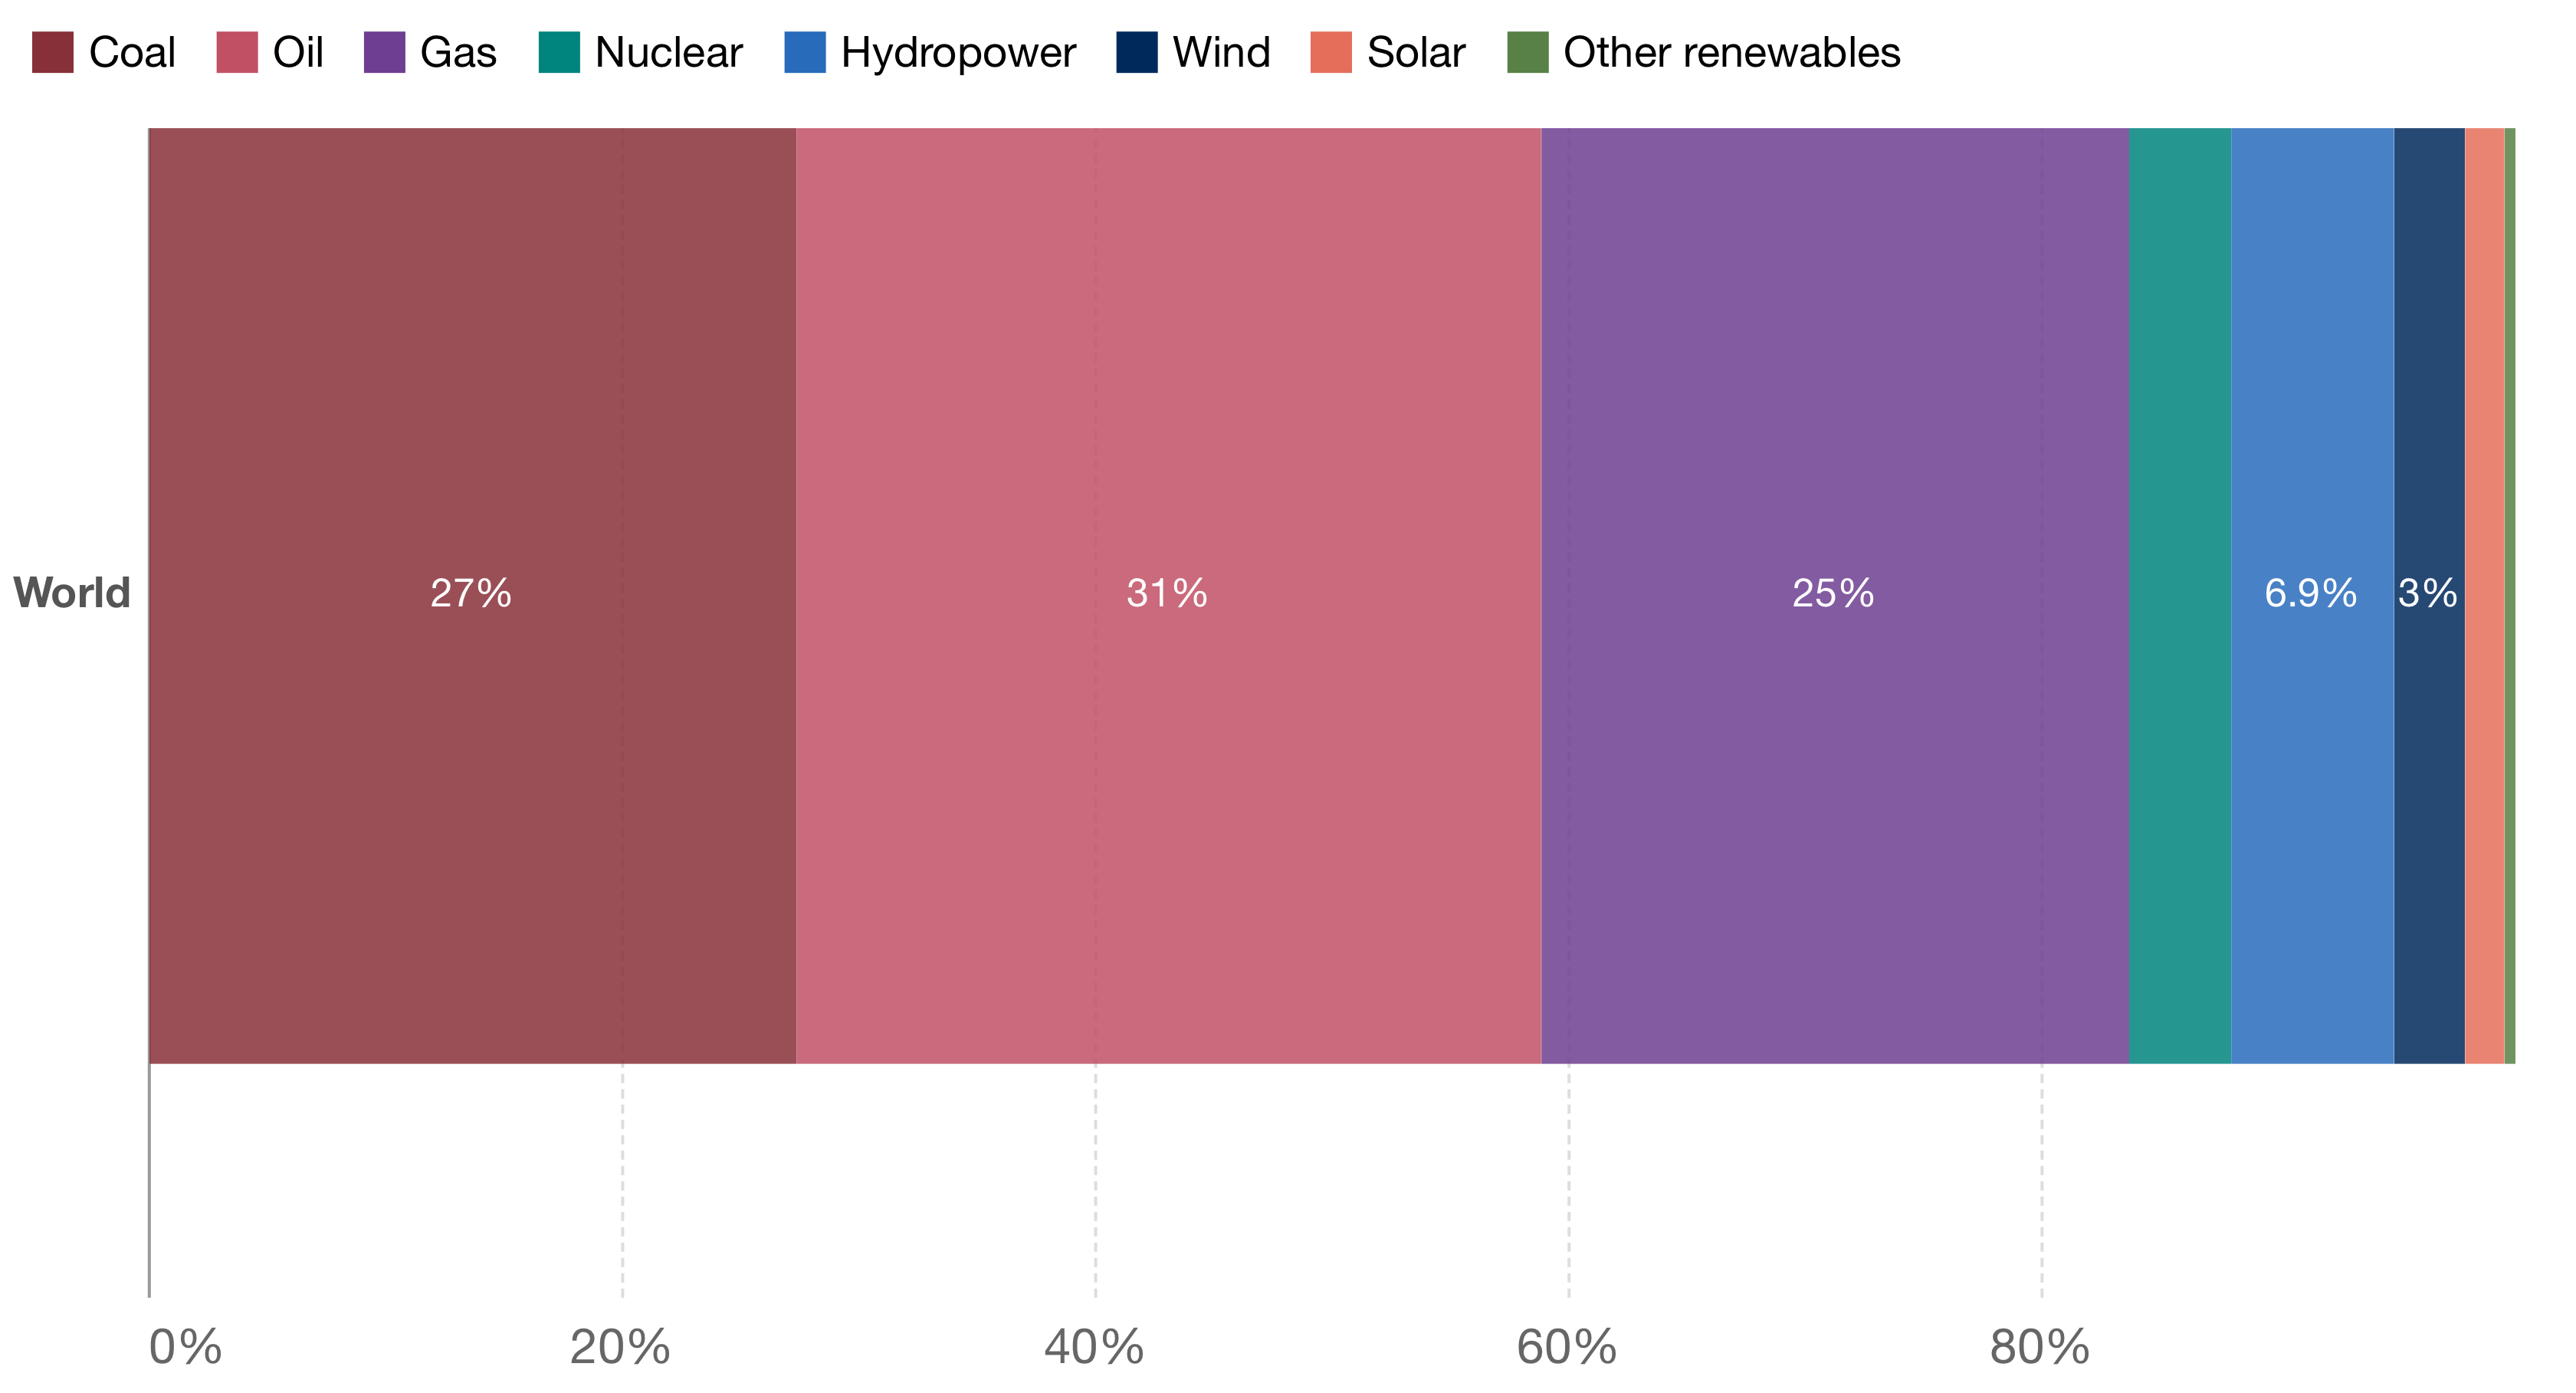
\includegraphics[width=\linewidth]{images/primary-energy-source-bar.png}
    \caption{Global energy consumption by source \citep{ritchieWhichSourcesDoes2021}.}
    \label{fig.energy consumption}
\end{figure}

The second class of energy source is the fossil fuels, such as coal, oil and natural gas. These fuels are formed from the remains of plants and animals over millions of year. Once extracted, these fuels can be burnt to generate generate electricity, power motors, or, in the case of oil, can be used as raw material for a wide variety of products, including plastic, chemicals and pharmaceuticals. These energy sources, thanks to their high power density, powered the industrial revolution, and are the foundation of our civilization in the 21st century. These energies do not suffer from the same shortcomings as renewable energy source --- they are not intermittent, and can easily be turned on and off to follow the demand. They however have many downsides. First and foremost, being non-renewable, there is only a limited amount of fossil fuels on Earth, which will eventually run out. Even if all disadvantages of fossil fuels are somehow avoided, humanity will have to move away from an economy based on fossil fuels because of their limited amount. Another disadvantage is that the consumption of fossil fuels is one of the main source of greenhouse gases, which contribute to global warming and climate change. Fossil fuels are not globally well distributed, which is the cause to numerous geopolitical instabilities in the world. Given the known reserves and the worldwide consumption of fossil fuels in 2020, humanity will exhaust supplies of coal in 139 years, of oil in 54 years, and of gas in 49 years \citep{bpBPStatisticalReview2020}.

Another class of energy source is nuclear energy. Today, nuclear power plants produce electricity by leveraging the nuclear fission of Uranium. Fission power plants operation do not generate any greenhouse gases, are not intermittent, and are routinely used to generate electricity for base-load consumption. The Uranium is however not well distributed globally, and is mainly being mined in Kazakhstan, Canada, Australia and Niger. Again, as for fossil fuel, this uneven distribution of resources is the source of geopolitical instabilities. Uranium is not renewable, and the world will eventually run out of fuel. According to the World Nuclear Association \citep{worldnuclearassociationUraniumSuppliesSupply2022}, the world's current annual consumption of uranium is around 61,000 metric tons. If this rate of consumption were to continue, the known land resources of uranium would last for around 90 years . However, this is a very rough estimate and does not take into account a number of factors that could affect the availability and use of uranium, such as the development of breeder reactors, changes in demand for electricity, or the exploitation of sea-water uranium ($4.6$ billion tons of uranium) \citep{dunganUraniumSeawaterInfinite2017}. Fission power plants generate long-lived nuclear wastes dangerous for living organisms. The risk of loss of control of the power plant, such as during the infamous accident of Chernobyl and Fukushima, can lead to catastrophic releases of nuclear material in the atmosphere. New power plant designs, with smaller amount of fissing materials in their core, and additional safety measures, can however make their use safer.  Despite these disadvantages, fission power plants are today the only energy source that can generate the amount of energy our civilization consumes without releasing greenhouse gases and without the inherent variability of renewable energies.

There are thus three pathways for future energy production: either massive structures are built across the globe to generate enough renewable energy, or massive funding is invested in developing and constructing new generations of fission nuclear power plant. The final pathway is exploiting a new source of energy that has not been discussed in the above discussion: \emph{nuclear fusion}. The advantages of nuclear fusion as a source of energy are numerous: the reaction does not generate any greenhouse gases, and, as for fission power and fossil fuels, is not intermittent. The considered fuel is Deuterium and Tritium, two isotopes of Hydrogen. Deuterium can be found in sea water, at a concentration of 155 part per millions (ppm), and is commonly extracted. Tritium is found in extremely small quantities on Earth, but can be produced by exposing lithium to a neutron flux,
\begin{equation}
    \ce{^{6}_{3}Li + ^{1}_{0}n -> ^{4}_{2}He + ^{3}_{1}T}.
\end{equation}
Lithium 6 is found in natural lithium, at a concentration of $7.5\%$. Though lithium is not equally distributed on Earth, extraction from seawater \citep{ZHAO2019113389} could be a future solution to this issue. Nuclear fusion does not face the same problematic as nuclear fission regarding nuclear wastes, as the reaction does not produce any radioactive materials. The reactor itself, exposed to neutron fluxes, is activated, and its materials have to be securely stored once decommissioned. These nuclear wastes are however short-lived in comparison to the nuclear wastes generated by nuclear fission. Finally, nuclear fusion reactors are intrinsically safe, as the reaction is not a chain reaction, and thus cannot undergo a core meltdown as nuclear fission reactors. Nuclear fusion comes also with a few disadvantages. As of today, the proposed reactor prototypes are large and expensive to build, and require a large upfront investment. Reaching the conditions for fusion is extremely difficult, and there are no reactor concept that has yet proven a net production of electricity. The National Ignition Facility (NIF) recently achieved a net power gain \citep{nif_source} on the fusion fuel, but is still far from a net energy gain when taking into account all the power plant energy consumption.

\section{Nuclear fusion as a source of energy}
Nuclear fusion is the process of forming a nucleus from two, lighter nuclei. This is the process that powers all stars in the universe, and that will power future fusion nuclear reactors. Nuclear \emph{fusion} is the opposite of nuclear \emph{fission}, where two nuclei are formed by breaking one, heavier nucleus, which is commonly used to power today's nuclear fission power plants.

Atomic nuclei are composed of neutron and protons, and are kept bound together by the strong interaction. The binding energy of the nucleon, defined as the minimum energy required to separate a nucleus as a collection of its nucleon, measures then how tightly bound a nucleus is. The binding energy per nucleon, shown on Figure \ref{fig. binding energy}, is low for hydrogen, grows with atomic number until reaching a maximum for the iron, and then decreases with increasing atomic number. In general, fusing two nuclei lighter than iron will then release energy, and so does fissing one nucleus heavier than iron.

\begin{figure}
    \centering
    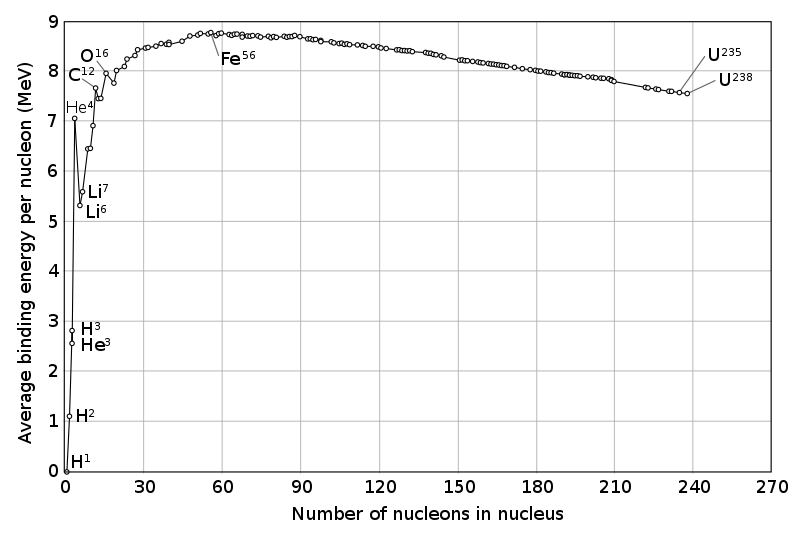
\includegraphics[width=.75\linewidth]{images/Introduction/BindingEnergy.png}
    \caption{Binding energy per nucleon. Credits: \url{https://tinyurl.com/4bmsrm3s}}
    \label{fig. binding energy}
\end{figure}

Of particular interest for commercial fusion power plants is the fusion of deuterium $\ce{H2}$ with tritium $\ce{H3}$, which generates a nucleus of helium $\ce{He4}$ with $3.5$MeV of kinetic energy, and a neutron with $14.1$MeV of kinetic energy (see Figure \ref{fig. dt fusion}). Among potential fusion reactions, this is the most promising, because the reaction cross-section is the highest. Nevertheless, deuterium-tritium fusion reactions require a temperature of at least $10$keV, \textit{i.e.} about 100 millions degrees. 
\begin{figure}
    \centering
    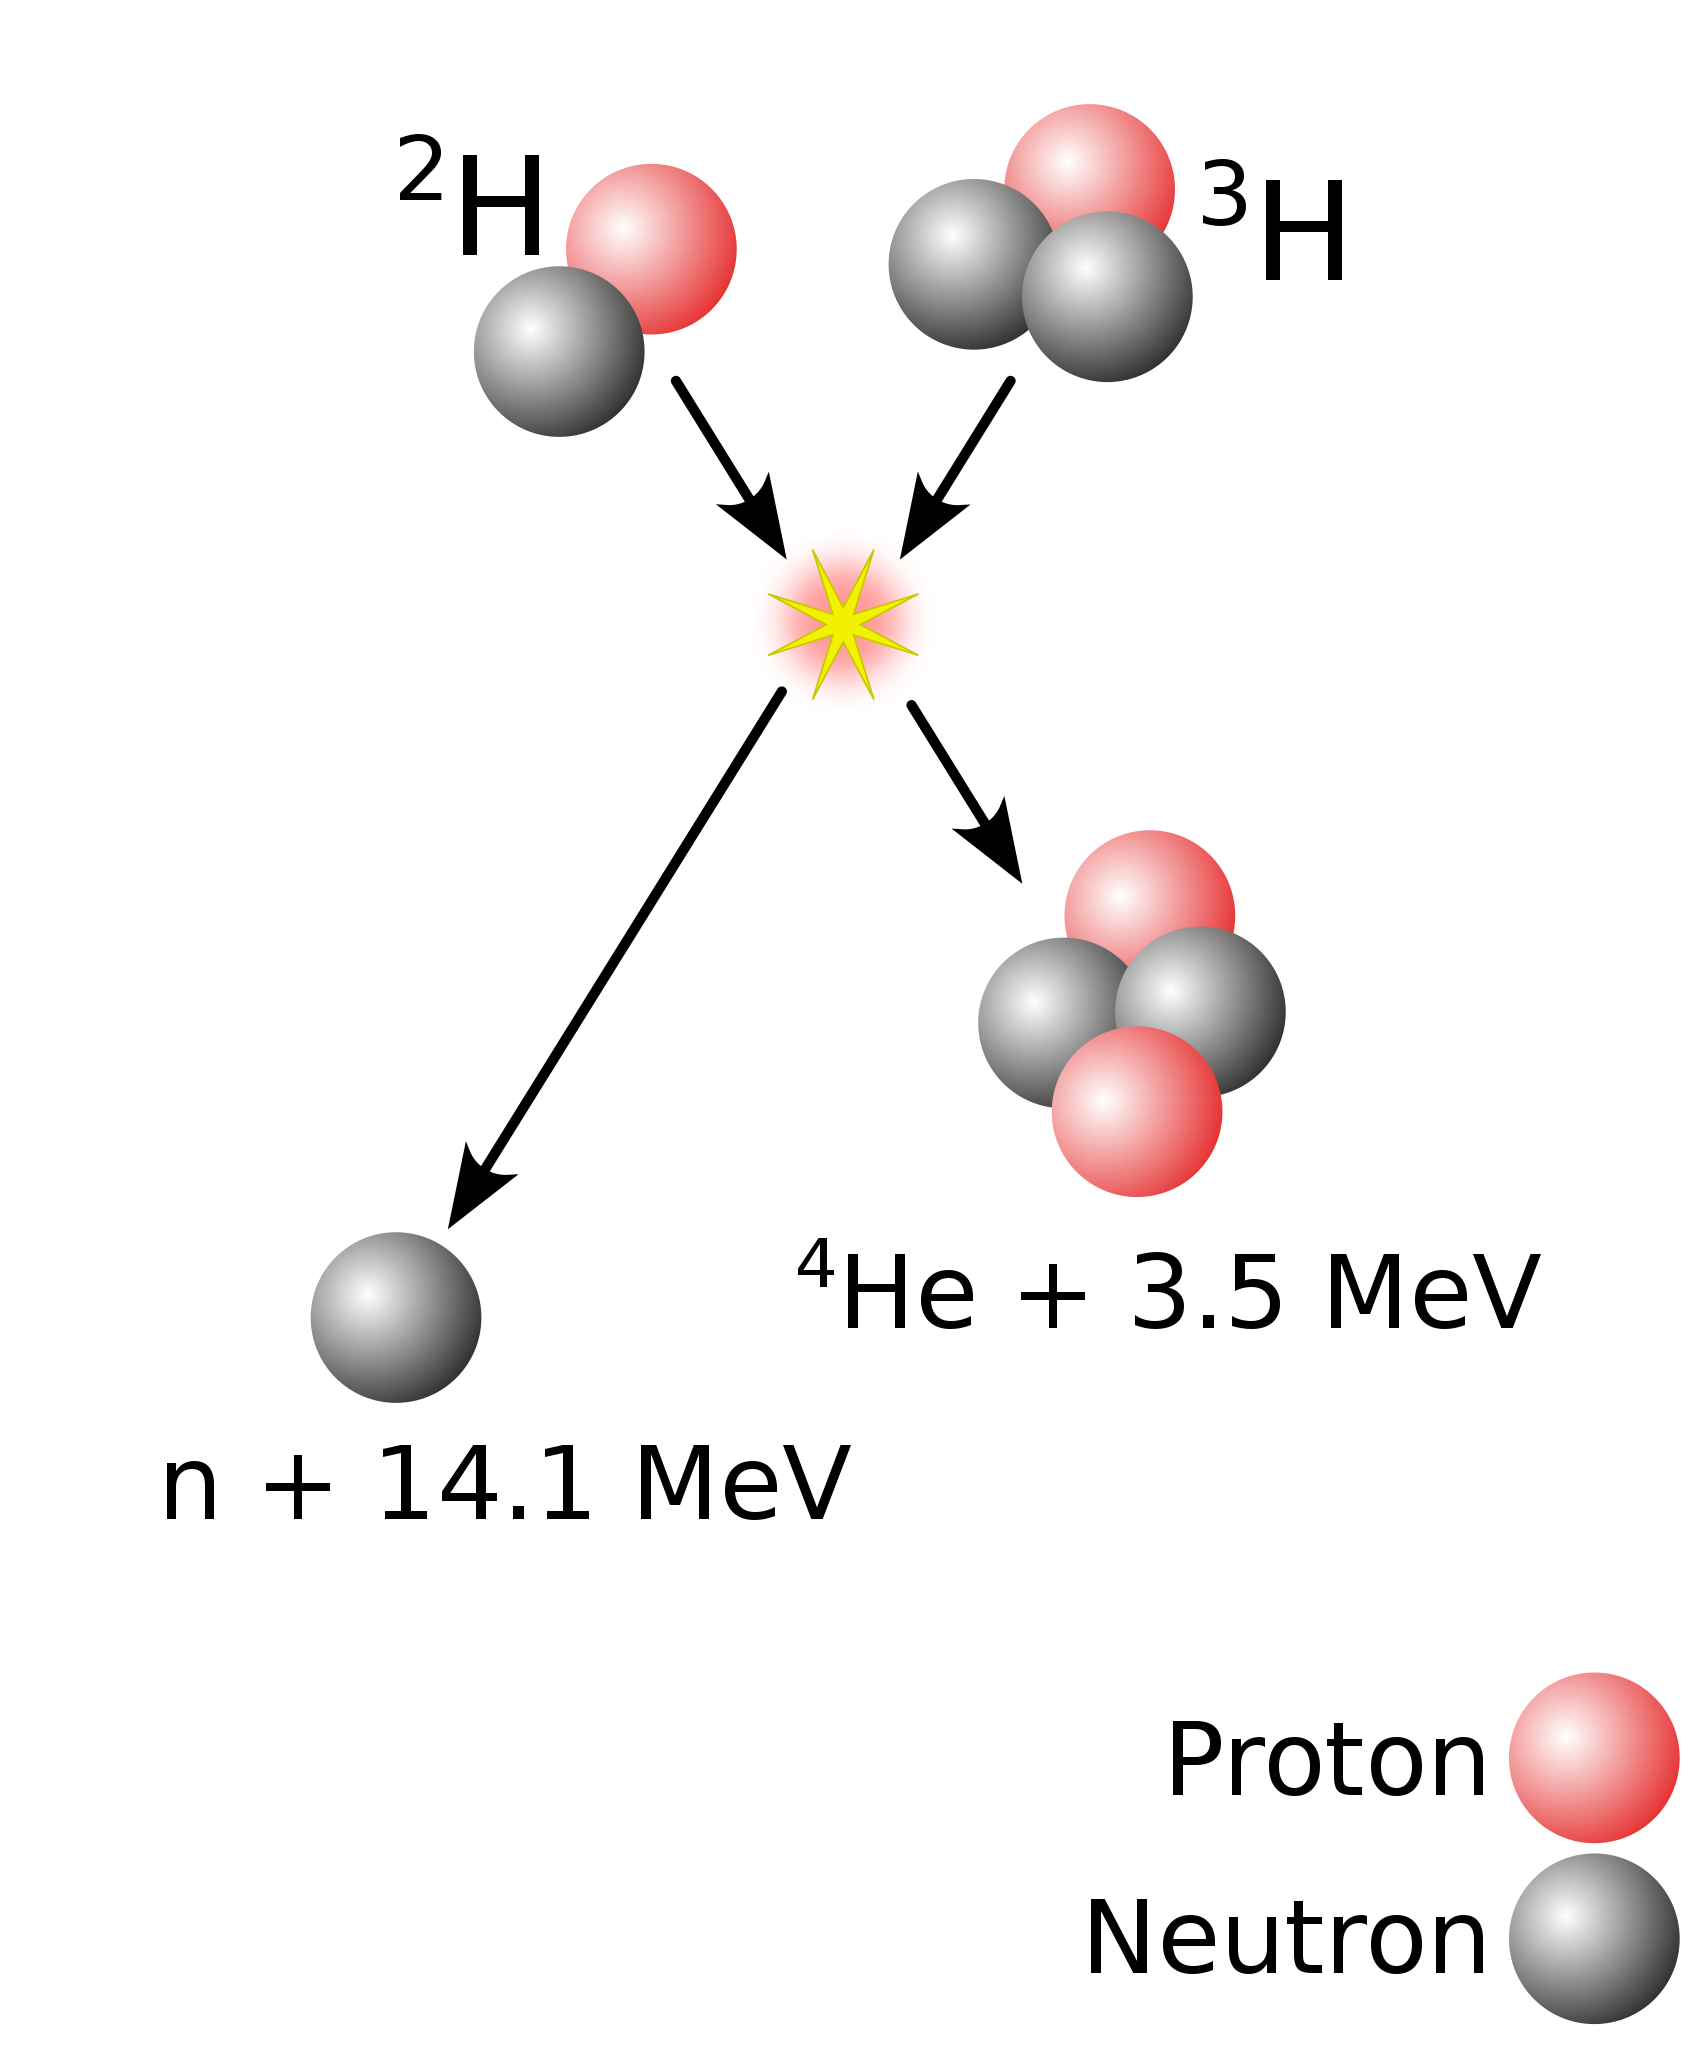
\includegraphics[width=.5\linewidth]{images/Introduction/DTFusion.png}
    \caption{Sketch of a Deuterium-Tritium fusion reaction. Credits: \url{https://tinyurl.com/3kyvakb4}}
    \label{fig. dt fusion}
\end{figure}

The challenge is then to confine the fuel, which is a plasma at these temperatures, for a sufficiently long time such that enough reactions have the time to occur. More specifically, we define the $Q$ factor as the ratio of power generated by the fusion reactions over the input power required to power the reactor, $Q=P_{fus}/P_{in}=1$. To get energy break-even, \textit{i.e.} to get as much fusion power as input power, $Q=1$, one can derive the so-called Lawson criterion \citep{lawsonCriteriaPowerProducing1957}, which gives a criterion on the fusion triple product,
\begin{equation}
    nT\tau_E > 1.5\cdot 10^{21}\text{keV s m}^{-3}, \label{eq. lawson criterion}
\end{equation} 
where $n$ is the plasma density, $T$ is its temperature, and $\tau_E$ is the energy confinement time. In addition, the plasma temperature cannot be too low nor too large, otherwise the fusion cross-section would be too small and Bremsstrahlung losses would fully compensate the generated fusion power. From the Lawson criterion \ref{eq. lawson criterion}, one can identify two paths toward a nuclear fusion power plant: (i) inertial fusion, where one maximizes the density for a very short amount of time, but does not confine the plasma, or (ii) magnetic confinement, where one keeps comparatively lower densities, but increases as much as possible the energy confinement time by confining the plasma using carefully designed magnetic fields. This thesis will focus on one particular design of magnetic confinement reactor called the stellarator, which we explain in the section \ref{sec.stellarator concept}.

First, the Virial theorem \citep{Freidberg2014} states that a plasma cannot generate a magnetic field to confine itself; an external magnetic field needs to be provided. To do so, one has to design a magnetic field which does not cancel anywhere in space --- otherwise the plasma would escape through this "hole" in the magnetic field. At first, one may think that the plasma can be shaped as a sphere. The hairy ball theorem \citep{Renteln2013-uu} however shows that there are no continuous tangent field that does not vanish anywhere on a sphere in 3-dimensional space. In fact, the only shape in 3D space with non-vanishing continuous vector field is a torus (or a klein bottle, but these are non-realistic shapes for a reactor). A magnetic fusion reactor must thus shape the plasma into a shape homeomorphic to a torus (see Figure \ref{fig.torus}).  In what follows, we will define the toroidal direction as the long way around the torus, and the poloidal direction as the short way around it.

\begin{figure}
    \centering
    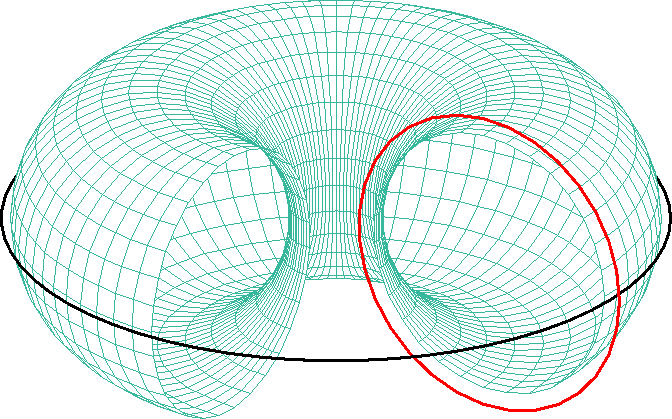
\includegraphics[width=.75\linewidth]{images/torus.png}
    \caption{Sketch of a torus. The red line follows the poloidal direction, while the black line follows the toroidal direction.}
    \label{fig.torus}
\end{figure}

\subsection{Single particle confinement in a torus}
In a magnetic field, single particles move freely along the magnetic field lines, and move in circles around the magnetic field line in the perpendicular plane. We say that the particle describe a gyromotion, with radius $\rho$ and frequency $\omega$, given by
\begin{align}
    \rho &= \frac{v_\perp}{\omega}\\
    \omega &= \frac{|q|B}{m},
\end{align}

{\color{red} add sketch of gyromotion with legend of rho, different velocities, ..}

where $v_\perp$ is the velocity of the particle perpendicular to the magnetic field line, $q$ is the charge of the particle, $B$ is the magnetic field strength, and $m$ is the particle's mass. The dynamics of single particles in a magnetic field can be greatly simplified if the magnetic field varies on scales larger than the gyroradius, $\rho|\nabla B|\ll B$, and that the magnetic field variations in time are much slower than a gyroperiod, $1/\omega \partial B/\partial t \ll B$. The equations of motion can then be averaged over a gyroperiod, and the motion of the particle is described by the trajectory of its guiding center.

We write the position of the particle as
\begin{equation}
    \mathbf{x} = \mathbf{r} + \rho\mathbf{s},\label{eq.single particle position}
\end{equation}
where $\mathbf{r}$ is the position of the gyrocenter, and $\mathbf{s}$ is a unit vector that rotate with the gyrophase $\gamma$. We require the gyroaverage of the second term on the right-hand side of Eq.(\ref{eq.single particle position}) to be zero, \textit{i.e.}
\begin{equation}
    \langle \rho\mathbf{s}\rangle_\gamma = \frac{1}{2\pi}\int_0^{2\pi} \rho\mathbf{s}d\gamma = 0,
\end{equation}
which means that the vector $\mathbf{r}$ is the gyroaveraged position $\langle\mathbf{x}\rangle_\gamma = \langle\mathbf{r}\rangle_\gamma = \mathbf{r}$. The particle velocity is then
\begin{equation}
    \mathbf{v} = \mathbf{u} + \frac{d\rho\mathbf{s}}{dt},
\end{equation}
with $\mathbf{v}=d\mathbf{x}/\mathbf{t}$ the particle velocity, and $\mathbf{u}=d\mathbf{r}/\mathbf{t}$ the guiding center velocity. Taking the equations of motion,
\begin{align}
    \frac{d\mathbf{v}}{dt} &= \frac{q}{m}(\mathbf{E}+\mathbf{v}\times\mathbf{B})\\
    \frac{d\mathbf{x}}{dt} &= \mathbf{v},
\end{align}
with $\mathbf{E}$ the electric field, one can show that the guiding center velocity in a electric and magnetic field at equilibrium (\textit{i.e.} time independent) can be written as a combination of three different drifts \citep{freidberg_2007},
\begin{equation}
    \mathbf{u} = \mathbf{V}_E + \mathbf{V}_{\nabla B} + \mathbf{V}_\kappa + u_\parallel \hat{\mathbf{b}},
\end{equation}
with $u_\parallel$ the velocity parallel to the magnetic field, $\hat{\mathbf{b}}=\mathbf{B}/B$, and
\begin{align}
    \text{The $\mathbf{E}\times\mathbf{B}$ drift}\qquad &\mathbf{V}_E = \frac{\mathbf{E}\times\mathbf{B}}{B^2}\\
    \text{The $\nabla B$ drift}\qquad &\mathbf{V}_{\nabla B} = \pm \frac{u_\perp^2}{2\omega}\frac{\mathbf{B}\times\nabla B}{B^2}\\
    \text{The curvature drift}\qquad &\mathbf{V}_\kappa = \pm \frac{v_\parallel}{\omega}\frac{\mathbf{R}_c\times\mathbf{B}}{R_c^2 B},
\end{align}
where the positive sign is taken for ions, the negative sign for electrons, $u_\perp$ is the guiding center velocity perpendicular to the magnetic field, and $\mathbf{R}_c$ is the curvature vector.

Let's assume that we construct a magnetic fusion reactor with a purely toroidal magnetic field, $\mathbf{B}= B\mathbf{e}_\phi$, where $\mathbf{e}_\phi$ is a unit vector in the toroidal direction. To generate such a field, toroidal coils with a coil current $I_c$ have to be used. Leveraging Ampere's law, we get $B \sim I_c / 2\pi R$, \textit{i.e.} the magnetic field is stronger close the torus hole, and smaller on the outer side of the machine, thereby defining a "high-field side" and a "low-field side" to the machine. In such magnetic field, a single particle will experience both a $\nabla B$ drift and a curvature drift in opposite vertical direction. In general, these drifts do not cancel each-others, and particles will drift in the vertical direction. Furthermore, because both drifts direction depends on the sign of the particle electric charge, electrons will drift in the opposite direction to the ions, and a charge separation will appear. A vertical electric field will emerge, which, thanks to the $\mathbf{E}\times\mathbf{B}$ drift, will push the particles outside the torus, thereby losing confinement. A purely toroidal magnetic field is thus not sufficient for confining a plasma.

{\color{red} add sketch of drifts in a purely toroidal magnetic field}

Adding a poloidal component to the magnetic field solves this problem --- due to their motion parallel to the magnetic field lines, particles will move from the upper portion of the torus to the lower one, and vice versa, which prevents the charge separation to occur, stops the electric field to emerge, and ultimately provides confinement within the torus to the particles. A magnetic field with a poloidal component wraps around the torus both in the poloidal and toroidal direction. This magnetic field line twist is described mathematically by the \emph{rotational transform}, which counts how many poloidal turns a magnetic field line does per toroidal turn. 

The rotational transform can be generated by three mechanisms \citep{Helander2014}: (i) driving a toroidal current in the plasma, or (ii) shaping the plasma as a rotating ellipse close to the axis, or (iii) having magnetic axis torsion. The tokamak, arguably the most advanced concept for a fusion reactor, uses uniquely the first mechanism. A strong toroidal current is driven in the plasma by an external transformer, and this produces the poloidal magnetic field (see Figure \ref{fig tokamak sketch}). One of its great advantage is that the configuration is axisymmetric --- \textit{i.e.} there are no dependencies on the toroidal position. This property of the tokamak, in particular, provides good neo-classical confinement, and, from an engineering point of view, makes it relatively simple to build. Driving such a strong current comes however with some disadvantages --- the operation of the machine is intrinsically pulsed, forbidding continuous operation of the machine and generating stress on the different components, and the current is a source of free energy in the plasma, which can generate powerful instabilities that have to be controlled. The stellarator, on the other hand, uses all three mechanisms to generate the rotational transform. We describe the stellarator concept, its advantages and inconvenient, in the next section.


\begin{figure}
    \centering
    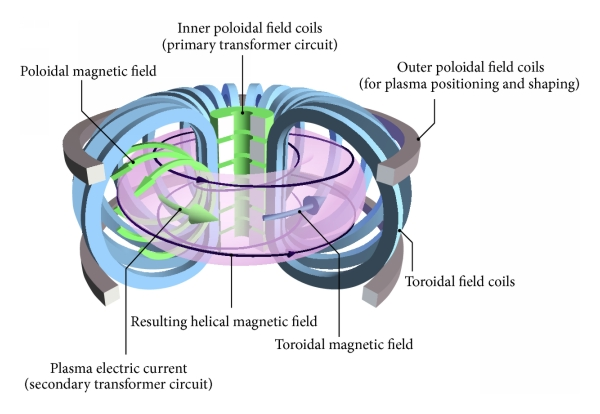
\includegraphics[width=\linewidth]{images/Introduction/TokamakSketch.jpg}
    \caption{Schematic of a tokamak. Credits: \url{https://tinyurl.com/bdfn3tc7}}
    \label{fig tokamak sketch}
\end{figure}


\subsection{The stellarator concept} \label{sec.stellarator concept}
The stellarator is a magnetic confinement device concept, that is homeomorphic to a torus. The stellarator, on the other hand, uses all three possibilities to generate the rotational transform. In practice however, the generation of a toroidal current is not considered, to not have the problems of the tokamak. These mechanisms comes at the cost of axisymmetry: the configuration is now fully 3-dimensional (see Figure \ref{fig stellarator sketch}). The physics, and engineering, are more complex, and extensive additional optimization is required to obtain neo-classical confinement of the same order as the tokamak. The plasma is however subject to less instabilities, and in general is much easier to operate experimentally. To summarize the comparison between the tokamak and the stellarator, one could say that the tokamak is easy to build but hard to operate, while the stellarator is hard to build but easy to operate.

\begin{figure}
    \centering
    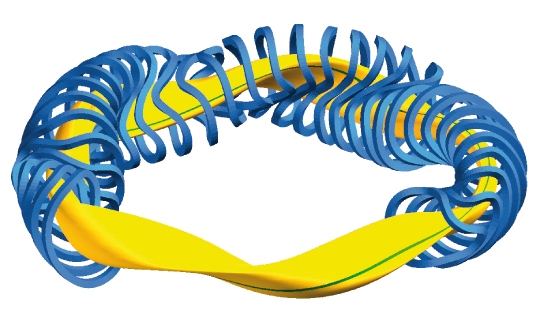
\includegraphics[width=\linewidth]{images/Introduction/StellaratorSketch.jpg}
    \caption{Schematic of a stellarator. Credits: \url{https://tinyurl.com/5ppm845w}}
    \label{fig stellarator sketch}
\end{figure}




\section{Magnetic field line topologies}

We discuss here the phenomenology of magnetic field equilibrium, and what kind of field line topologies exist in 3D equilibria. Three dimensional magnetic fields are, in general, composed of  magnetic surfaces, magnetic islands and magnetic field line chaos (see Figure \ref{fig. topology examples}). Measurements in the Wendelstein-7X stellarator via injection of an electron beam in a dilute gas \citep{pedersenConfirmationTopologyWendelstein2016} showed experimentally the existence of magnetic surfaces (Figure \ref{fig w7x magnetic surface}) and of the edge magnetic island chain (Figure \ref{fig w7x magnetic island}).

\begin{figure}%
	\centering
	\subfloat[Magnetic surface]{\label{fig w7x magnetic surface}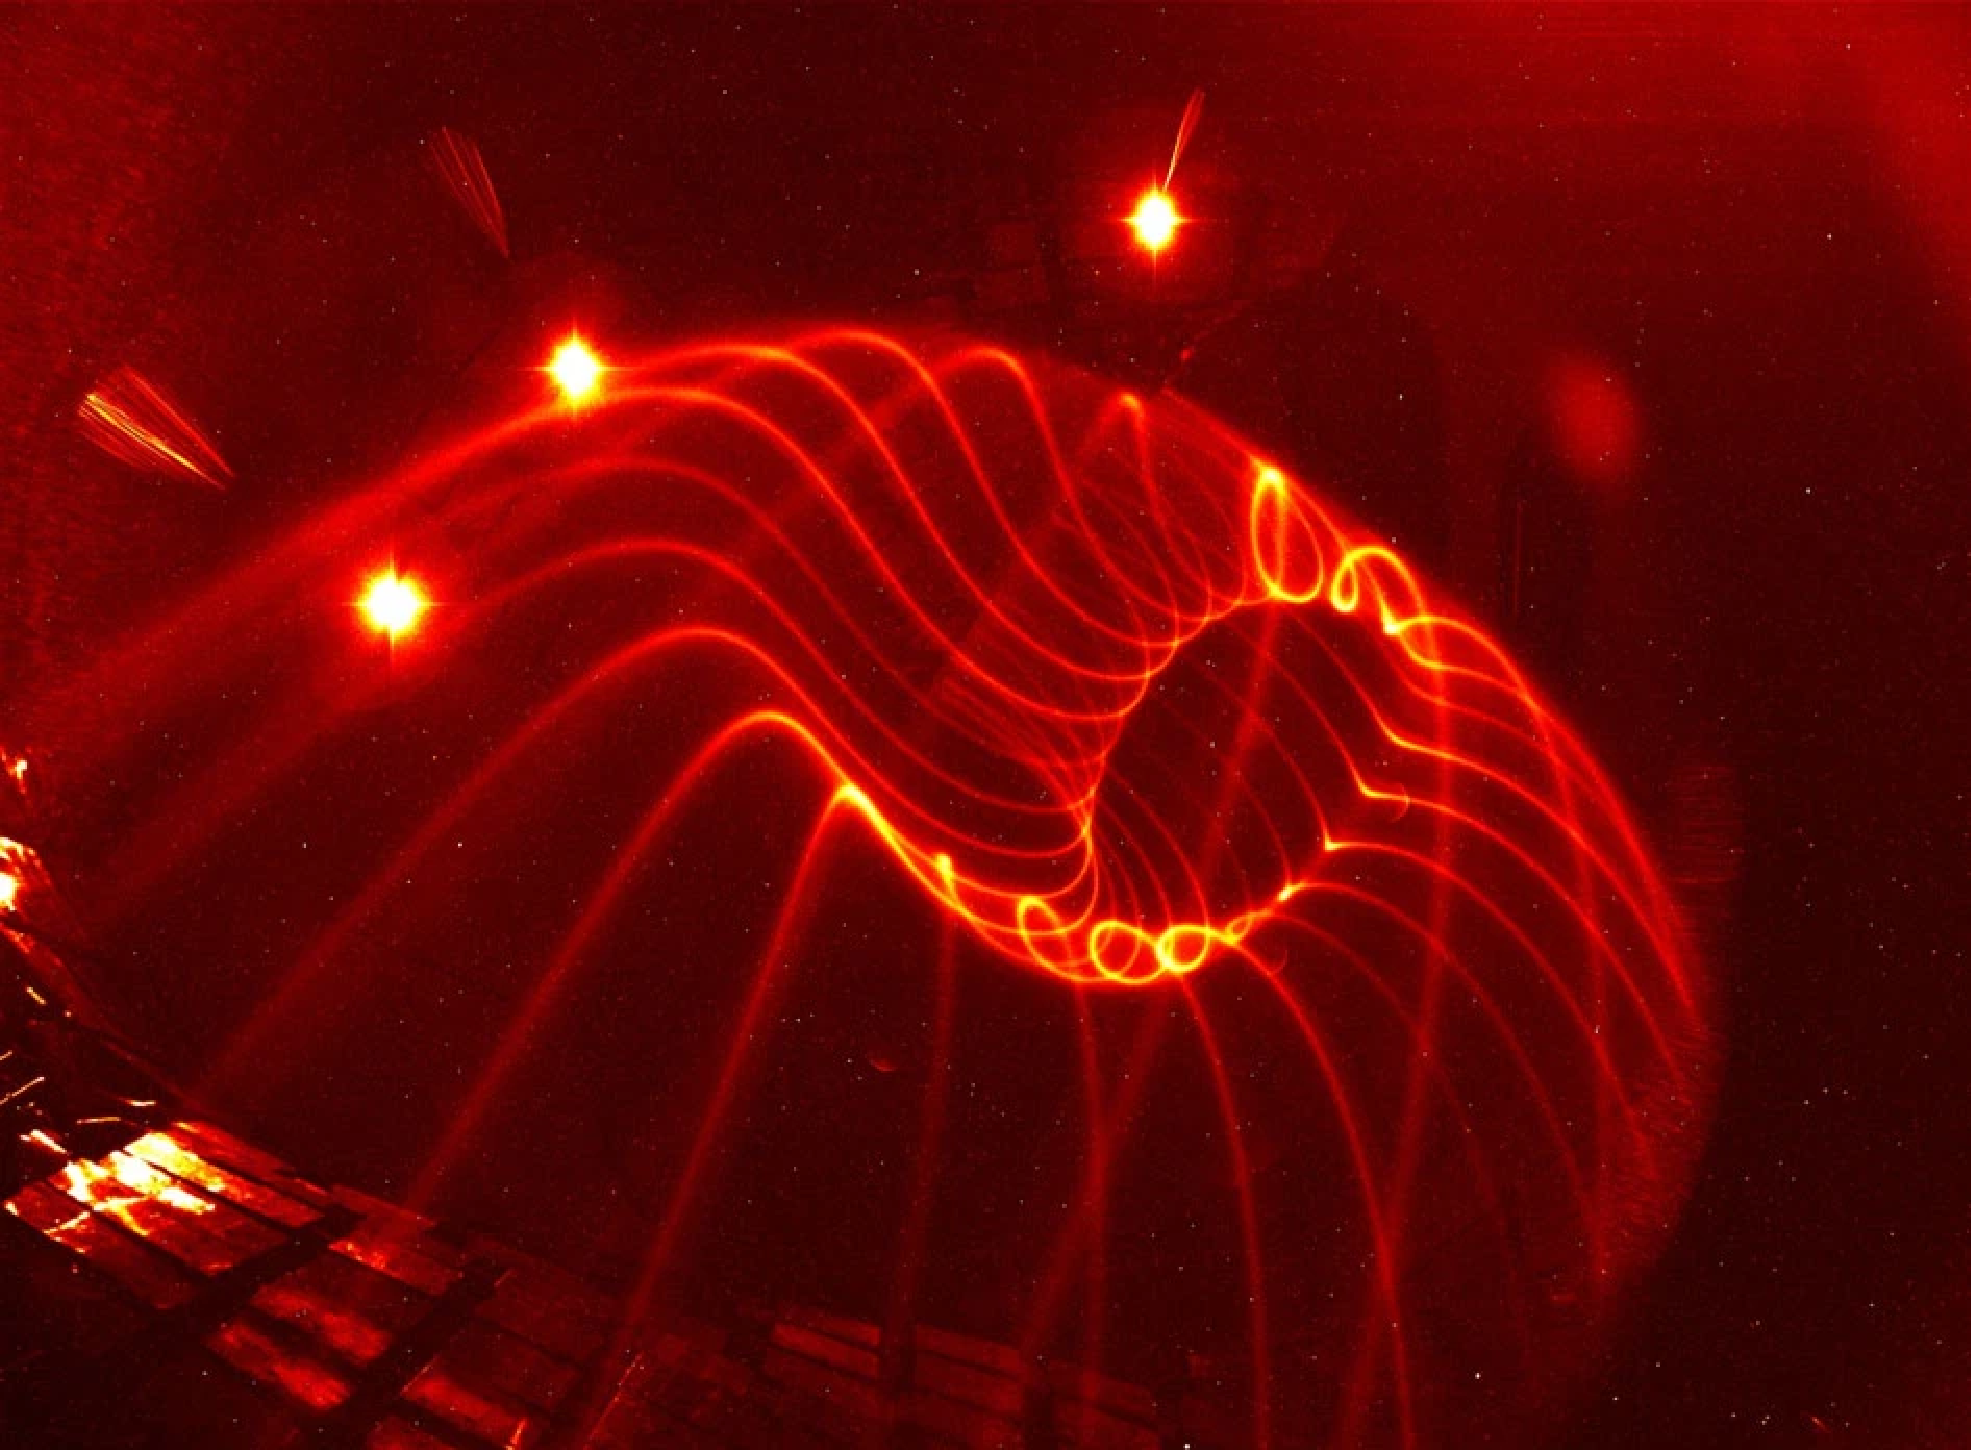
\includegraphics[height=4.8cm]{images/Pedersen2016_MagneticSurface_W7X.pdf}}%
	\qquad
	\subfloat[Magnetic islands]{\label{fig w7x magnetic island}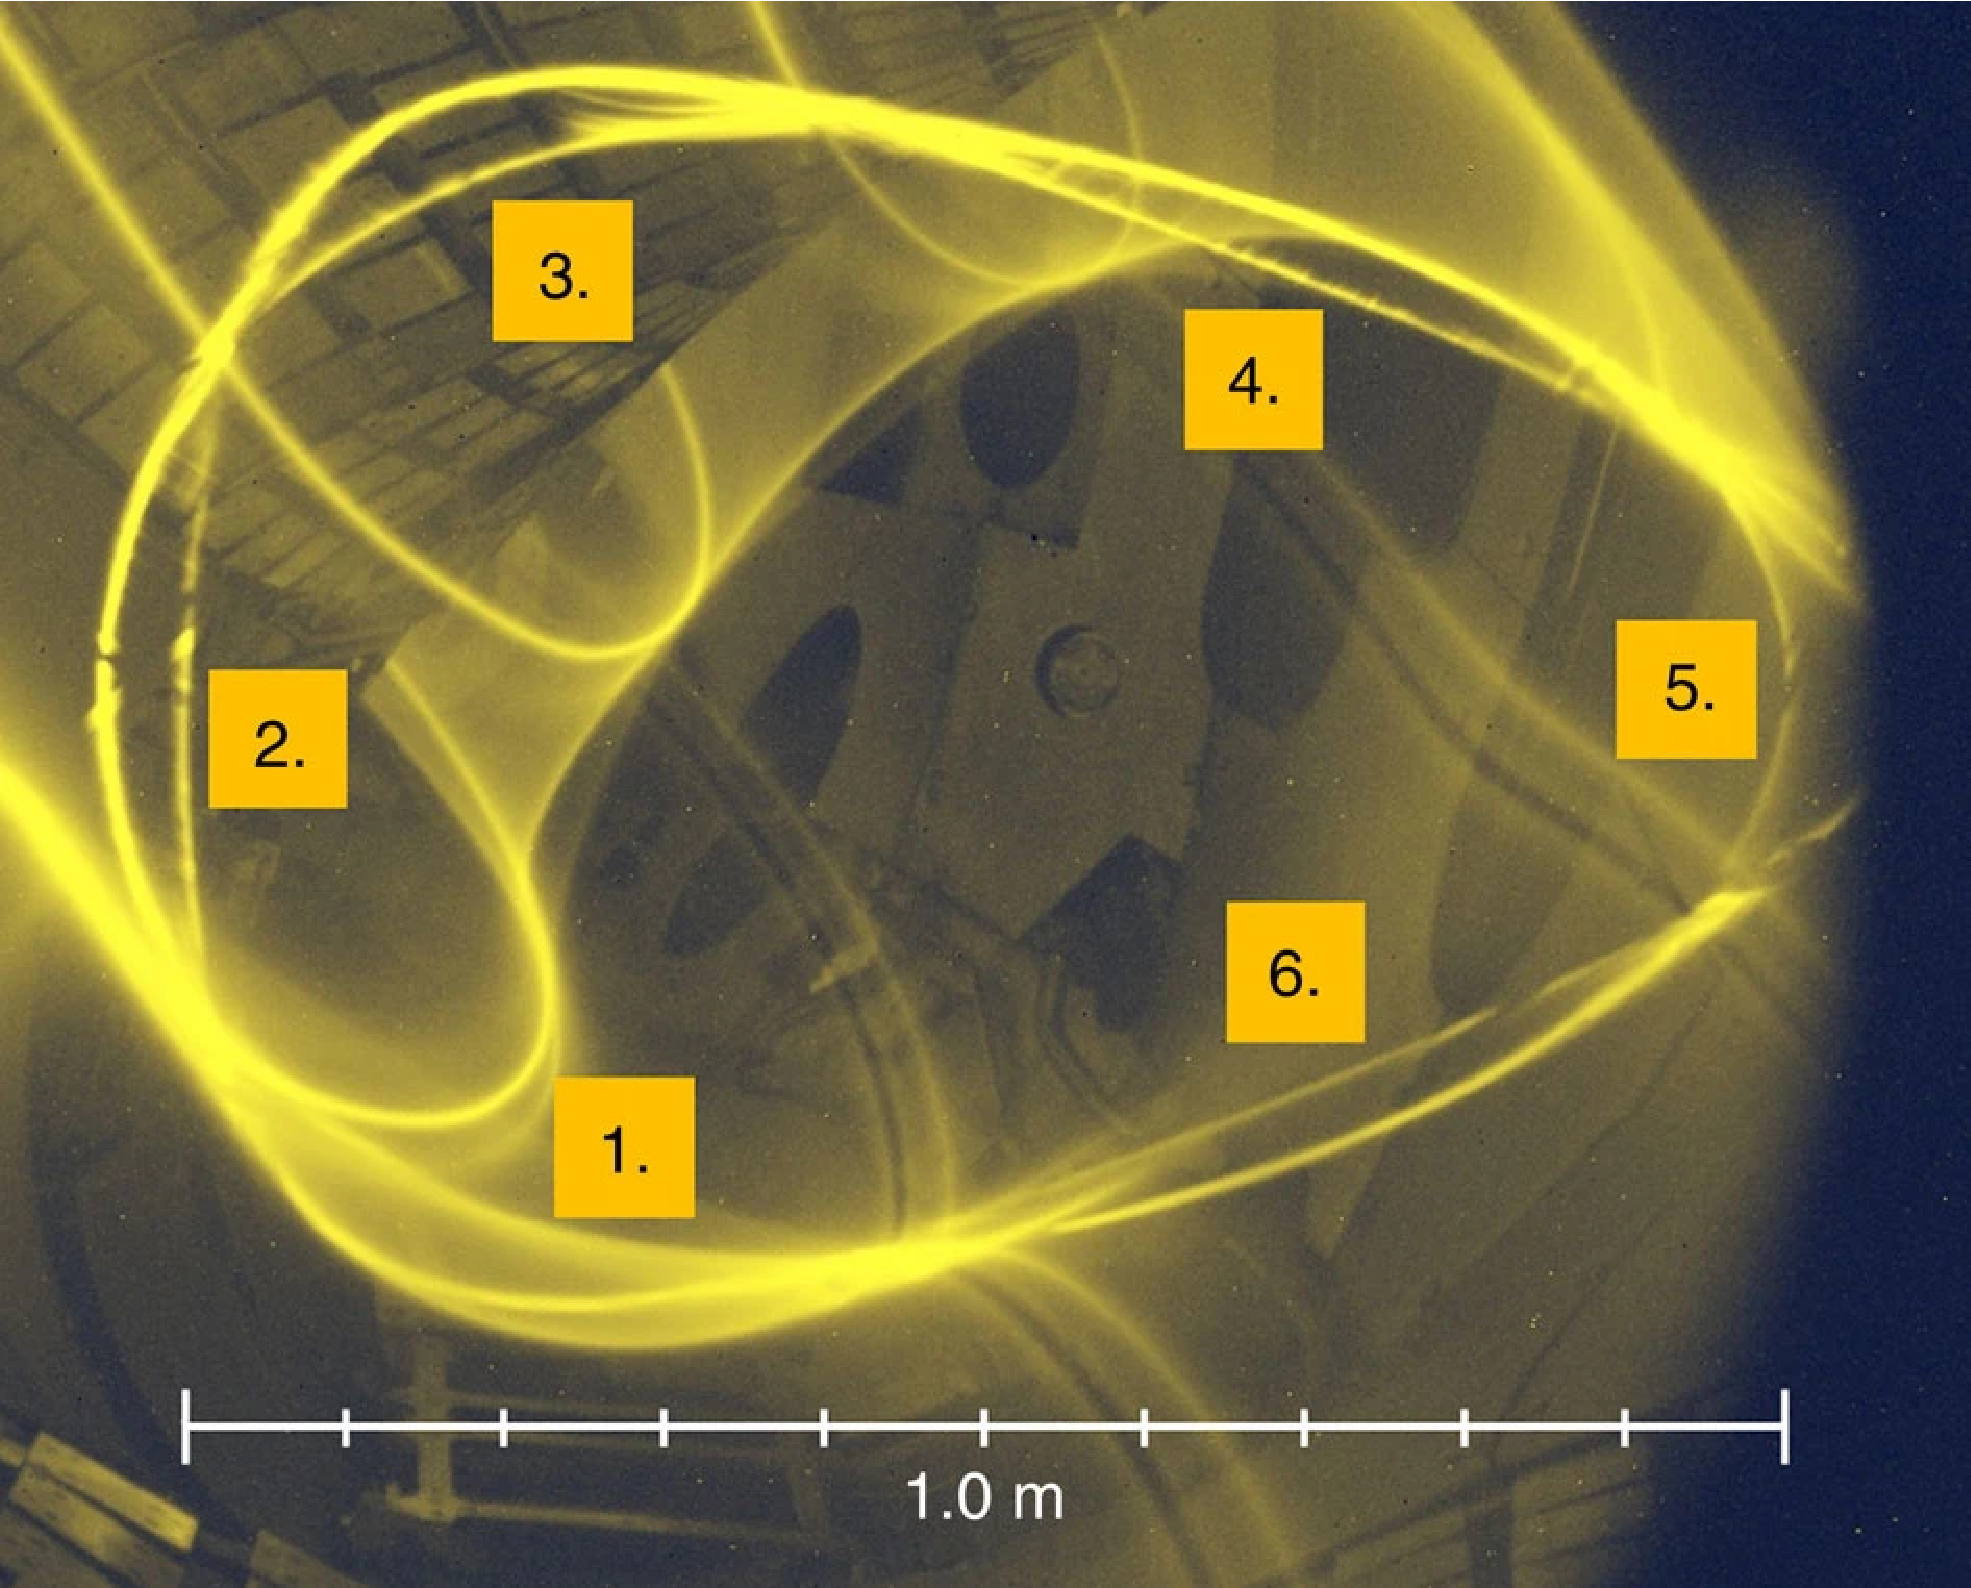
\includegraphics[height=4.8cm]{images/Pedersen2016_MagneticIsland_W7X.pdf}}
	\caption{Measurement of the field line topology in W7-X via injection of an electron beam in a dilute gas \citep{pedersenConfirmationTopologyWendelstein2016}.}
	\label{fig. w7x topology measurement}%
\end{figure}

Now, suppose that an equilibrium is given --- by that, we mean that the magnetic field $\mathbf{B}$ is known everywhere, \textit{i.e.} at any position $(r,\theta,\phi)$, where r is a radial coordinate, $\theta$ is a poloidal angle and $\phi$ is the usual cylindrical toroidal angle. To visually see the magnetic field line topologies, a Poincare section can be plotted. To do so, the field line is followed by solving the differential equation
\begin{equation}
	\frac{d\theta}{d\phi} = \frac{\mathbf{B}\cdot\nabla\theta}{\mathbf{B}\cdot\nabla\phi},
\end{equation}
with initial condition $r(0)=r_0$, $\theta(0)=\theta_0$ where $(r_0,\theta_0)$ are the initial field line position at $\phi=0$. An example of a field line followed on a magnetic surface is shown on Figure \ref{fig. field line tracing}. The field line is followed for multiple toroidal transits, and its position $(r_k,\theta_k)$ is saved whenever $\phi=2k\pi$, with $k\in\mathbb{N}$. The Poincare section is then plotted on the $(R,Z)$ plane. An example of a Poincare section with different field line topologies is shown on Figure \ref{fig topology examples}.

\begin{figure}
	\centering
	\subfloat[][Field line]{\label{fig. field line tracing}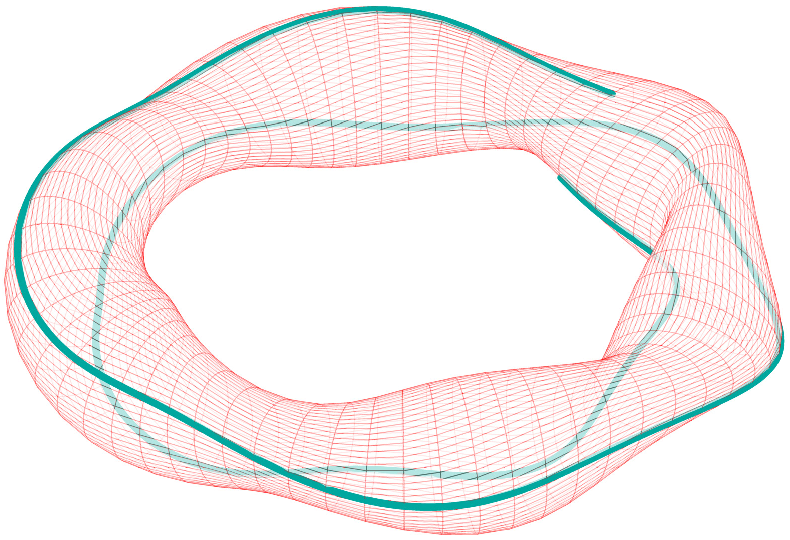
\includegraphics[height=4cm]{images/3d_field_line_tracing.pdf}}
	\hfill
	\subfloat[][Poincare section]{\label{fig. topology examples}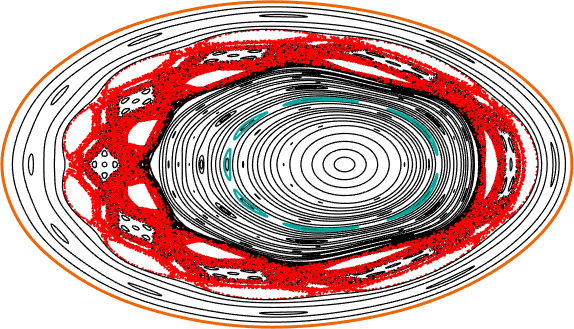
\includegraphics[height=4cm]{images/poincare_section_example.pdf}}
	\caption{Example of field line tracing and Poincare section in a rotating ellipse. Left: 3D mesh of a magnetic surface (red) and a traced field line over two periods (blue). Right: Poincare section of multiple field lines, a magnetic surface (orange), a magnetic island (blue) and a chaotic field line (red).}
	\label{fig poincare section}
\end{figure}

%Magnetic surfaces are toroidal surfaces on which the magnetic lays, \textit{i.e.} $\mathbf{B}\cdot\mathbf{n}=0$ with $\mathbf{n}$ a vector normal to the magnetic surface. In axisymmetric devices such as tokamaks, one can prove that nested magnetic surfaces exist everywhere, from the plasma edge to the magnetic axis, which is the innermost field line. Magnetic islands are formed when (i) the magnetic field is perturbed with a mode $\delta B_r \propto exp(i(m\theta-n\phi))$, with $(\theta,\phi)$ a poloidal and toroidal angle, and $m$, $n$ the poloidal and toroidal mode number, and (ii) the rotational transform is a rational number equal to $\iotabar=n/m$. Finally, magnetic field line chaos is formed when two or more island chains overlap --- this is the so-called Chirikov criterion \citep{Chirikov1979}. Further details about these magnetic field line topologies and their hamiltonian description can be found in the review paper by \citet{Meiss1992c} and references therein. 

%To accurately model and understand the physics in a stellarator, it is important to consider equilibria that allow magnetic islands and magnetic field line topologies. In the following chapter, we discuss important properties of the ideal \ac{MHD} model (section \ref{section ideal mhd}), the Taylor relaxation model (section \ref{section taylor state}) and of the \ac{MRxMHD} model (section \ref{section mrxmhd}).

At zeroth order, particle and energy confinement is obtained on magnetic surfaces; magnetic islands and magnetic field line chaos, on the other hand, may increase radial transport. This is not the full story; structures in regions occupied by chaotic field lines can potentially support pressure gradient \citep{Hudson2008}, but in general the transport in these regions will be greater than in regions occupied by magnetic surfaces. We thus desire to design stellarators with a large volume occupied by magnetic surfaces. In vacuum, \citet{Hanson1984a,Cary1986} showed that magnetic islands and magnetic chaos could be systematically eliminated by carefully designing the external coils. Pressure driven currents will  however perturb the carefully designed vacuum magnetic field, and will generate magnetic island and magnetic field line chaos at finite pressure.

In this thesis, we explore the effects of the pressure-driven currents on the stellarator equilibrium. In particular, we want to implement new capabilities in the \ac{SPEC} code to compute free-boundary, finite pressure, finite current, 3-dimensional magnetohydrodynamic equilibria with magnetic islands and magnetic chaos. With this tool, we can then explore the breaking of magnetic surfaces as the plasma pressure and the pressure-driven currents increases. We want to model and extract critical parameters for the critical pressure at which the magnetic equilibrium starts to deteriorate, and explore what degree of freedom can be optimized to increase this critical pressure.

% \begin{figure}
% \centering
% 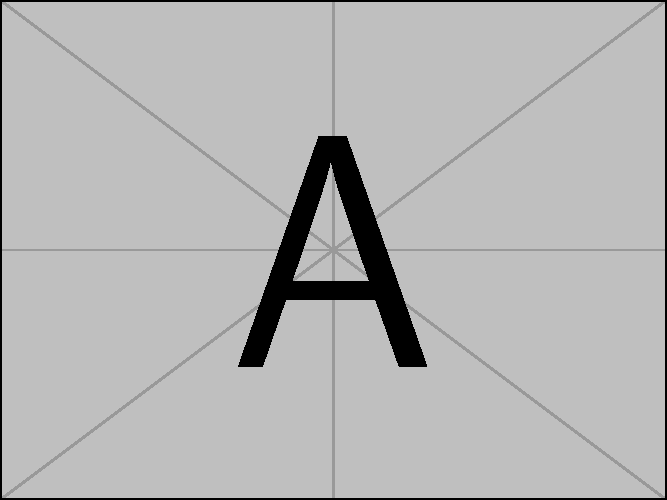
\includegraphics[width=\linewidth]{images/example-image-a.pdf}
% \caption{Example of a magnetic surface, a magnetic island chain and magnetic field line chaos.}
% \label{fig. topology examples}
% \end{figure}

%In the next sections, we will discuss different mathematical models that have been developed to describe 3D magnetic equilibria, \textit{i.e.} answering the question "\emph{Given a boundary, pressure and current profiles, what is the magnetic field in a plasma?}"

\end{document}


